\section{Data}
%\section{DICOM Data}

To visualize cardiovascular data we first had to search approprite data that exhibit the information we want to visualize. We refer here to DICOM and DAT files, as the former are relevant in medical visualization and the latter is our own format that is read by our application.

\subsection{DICOM}

In the field of medical visualization DICOM is the defacto standard for capturing, annotating and deploying data.
Including meta information and high dynamic range images DICOM is our preferred way to load medical data into our system.

\subsection{DAT}

The DAT format consists of 16 bit data chunks where the first three chunks provide the resolution of the volume in x,y and z-coordinate for uniform scaled voxels. The following data entries also consiste of 16 bit chunks where the values are are encoded as 12 bit values. 

\subsection{Data Acquisition}

To our disappointment we had to find out that it is rather difficult to find appropriate vascular data of the heart.


\subsection{Data Import}

One of the key advantages of DICOM data over simple image stacks is the fact that pixel intensities and radiometric intensities do not need to be the same in a given image stack. So DICOM provides a mapping to use several images together within a homogen radiometric background.


\begin{figure}[h]
	\centering
	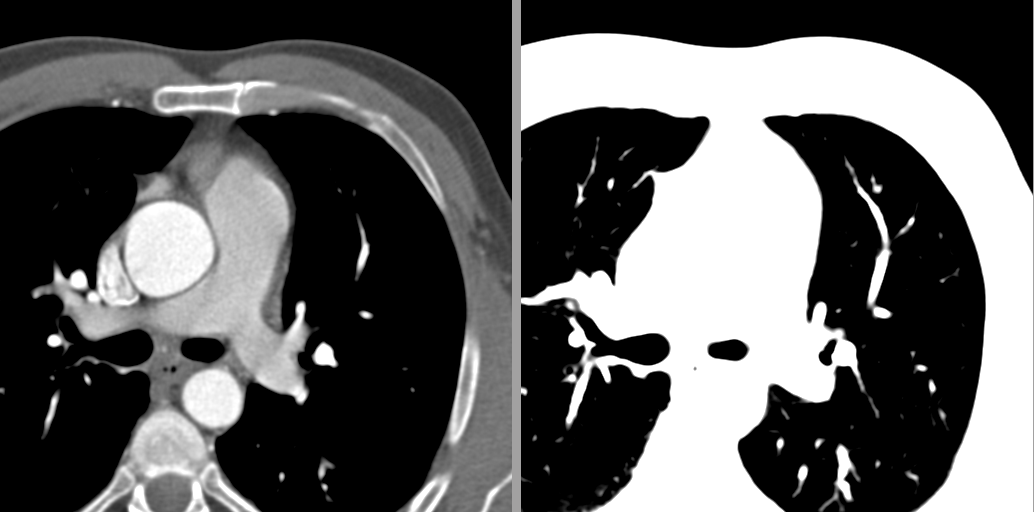
\includegraphics[width=0.45\textwidth]{IM-0001-0019_20.png} \\
	\caption{Stacked images with inhomogenous radiometric space. DIOCM sample data \emph{CARDIX} \cite{gimias_sampledata_2018} aquired from sample data section of the GIMAIS project \cite{gimias_2018} and processed with \emph{dicom2jpeg} from imbera project \cite{imebra_dicom_sdk_2018}.}
	\label{fig:IM-0001-0019_20}
\end{figure}

Simple exports of JPEG data out of DICOM without respecting this relation spills out images with are not homogenous across the stack as seen for instance in figure \ref{fig:IM-0001-0019_20}.


\subsection{Data Conversion}

As it was not possible to find a suitable DICOM reader for our \emph{CARDIX} dataset \cite{gimias_sampledata_2018} for VTK we used an intermediate step via MITK and convert DICOM data with the help of MITK main application to VTK 3D Image (VTI) data readable by VTK.
In this way we could overcome the problems with codecs and intensity differences across the image stack.

We write the data from VTI file format to our own DAT format that holds 12 bit intensity values in row major order where every data entry consists of an unsigned short, so 16 bit value. The first three entries describe the resolution of the dataset in x,y and z direction.

For the \emph{CARDIX} dataset we could convert the VTK image just with a regular rescaling of every data entry to our 12 bit range. For the \emph{MAGIX} dataset we had to resample the original dataset. As scanning resolution can differ according to the dimension, we rescaled our 3D datasets accordingly. 

Alternatively we also convert from PVM file format defined by Roettger et al.~\cite{roettger_PVM_2018} to visualize the \emph{Angio} dataset form the repository of \emph{The Volume Library}~\cite{roettger_VOL_2018} website. 

\subsection{Datasets}

Here we list the datasets we visualize to show the abilities of MIDA. 

\begin{figure}[h]
	\centering
	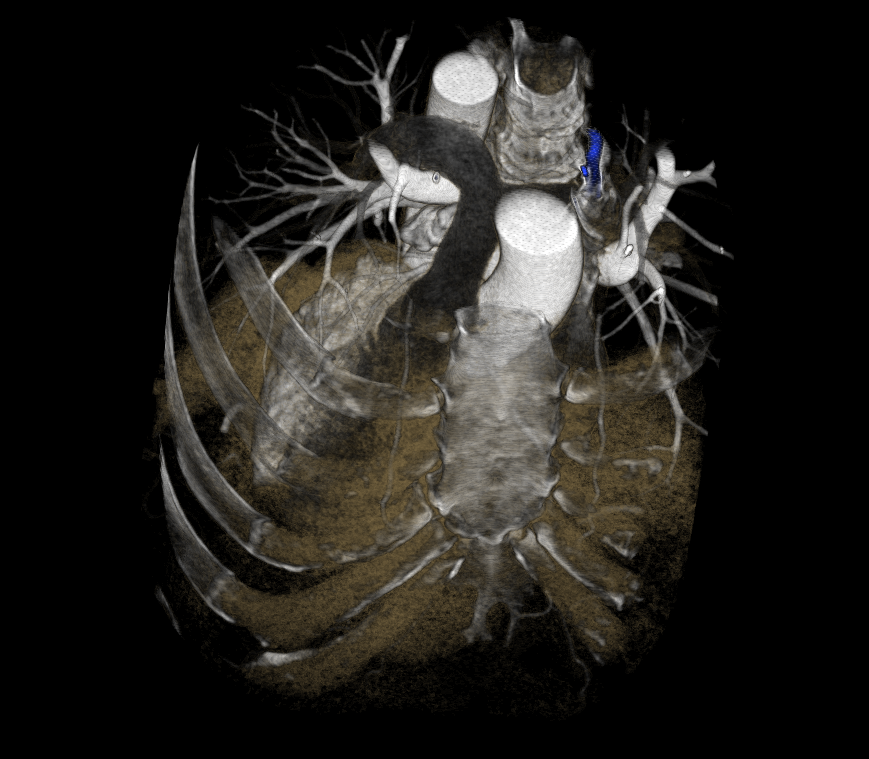
\includegraphics[width=0.45\textwidth]{VIS1_Alpha_CARDIX_02.png} \\
	\caption{DAT conversion from sample data \emph{CARDIX} \cite{gimias_sampledata_2018} aquired from sample data section of the GIMAIS project \cite{gimias_2018}.}
	\label{fig:Vis1_Alpha_CARDIX_02}
\end{figure}

\begin{figure}[h]
	\centering
	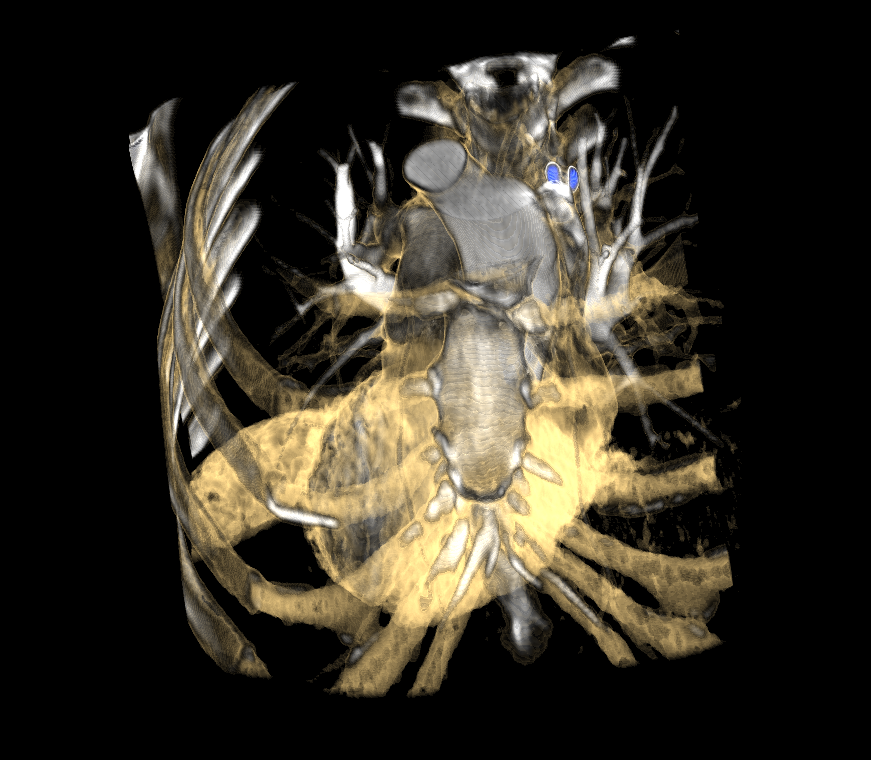
\includegraphics[width=0.45\textwidth]{VIS1_Alpha_MAGIX_05.png} \\
	\caption{DAT conversion from sample data \emph{MAGIX} \cite{gimias_sampledata_2018} aquired from sample data section of the GIMAIS project \cite{gimias_2018}.}
	\label{fig:Vis1_Alpha_MAGIX_05}
\end{figure}


\begin{figure}[h]
	\centering
	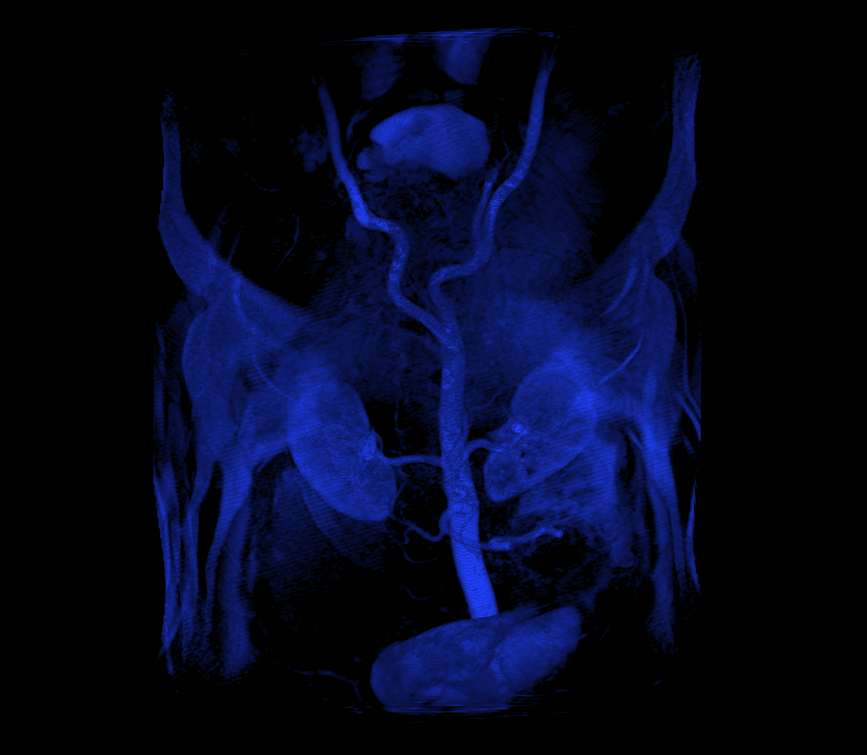
\includegraphics[width=0.45\textwidth]{VIS1_Alpha_Angio_02.png} \\
	\caption{DAT conversion from sample data \emph{Angio} \cite{roettger_VOL_2018} aquired from \emph{The Volume Library} website \cite{roettger_VOL_2018}.}
	\label{fig:Vis1_Alpha_Angio_02}
\end{figure}

Our datasets consist of \emph{CARDIAS} as shown in figure \ref{fig:Vis1_Alpha_CARDIX_02}, \emph{MAGIX} as shown in figure \ref{fig:Vis1_Alpha_MAGIX_05} and \emph{Angio} as shown in figure \ref{fig:Vis1_Alpha_Angio_02}.

